\section{Algorithm for planar fractures}
\label{section: Chapter4/algo}

\begin{figure}[h]
    \centering
    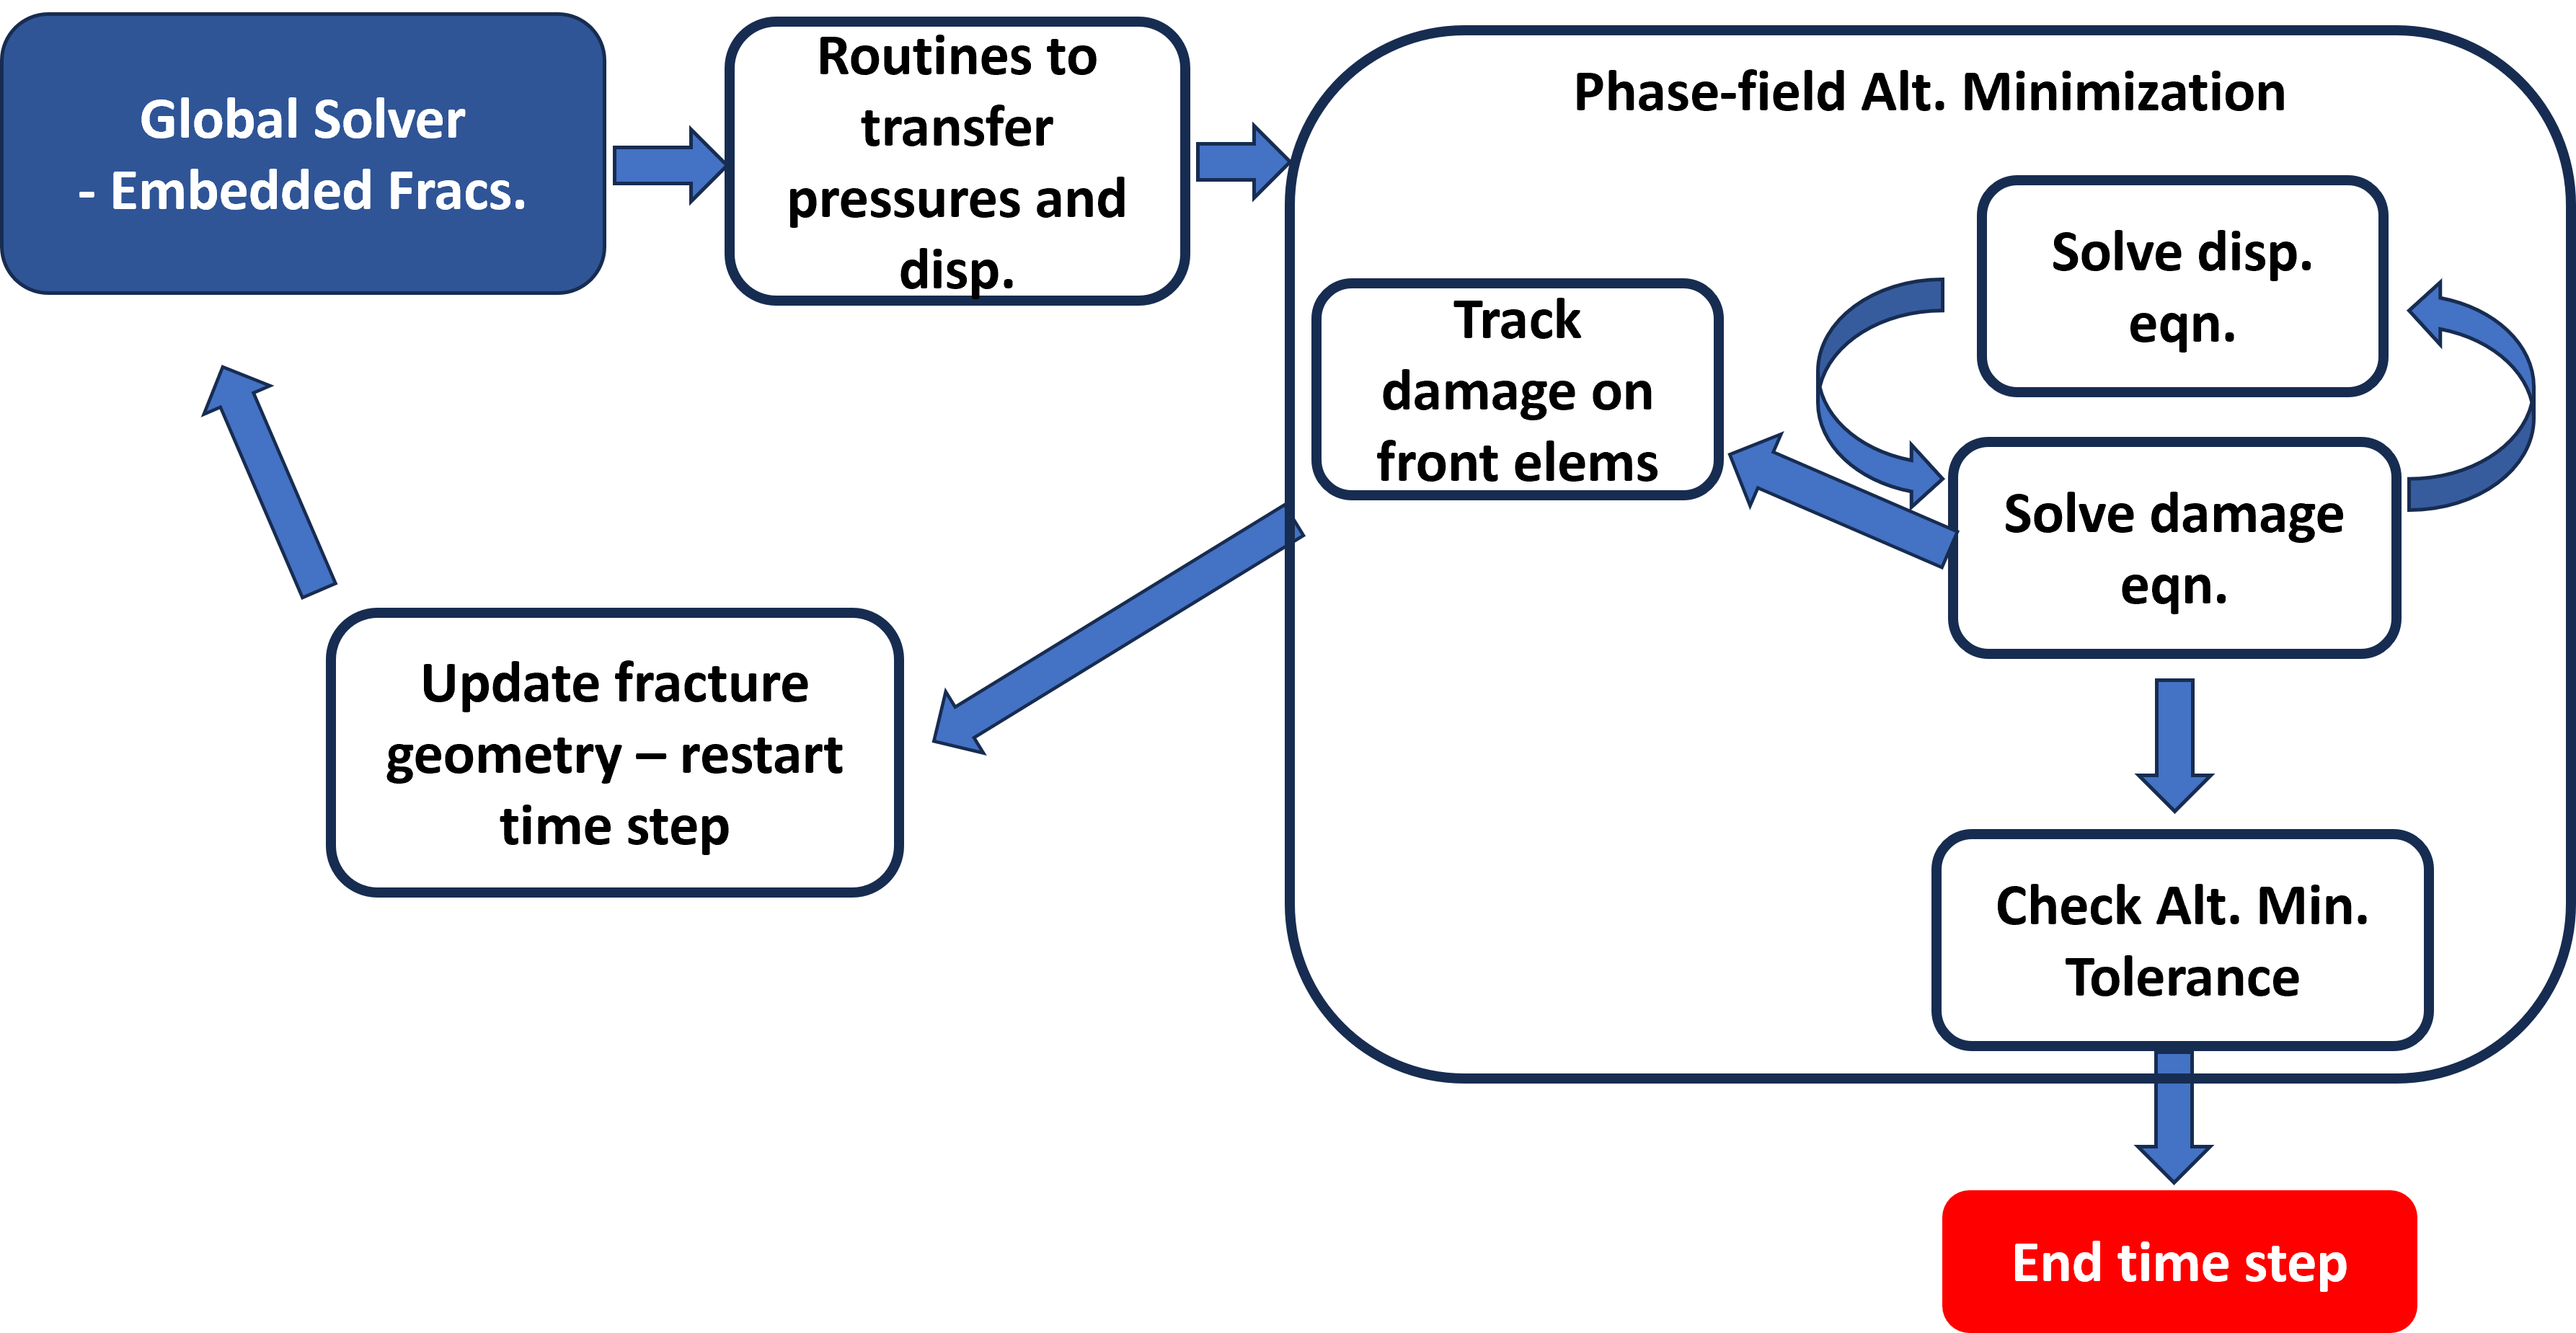
\includegraphics[width=\linewidth]{Chapter4/figures/planar3D_algorithm.png}
    \caption{Multi-resolution solution algorithm.}
    \label{fig:MR_planar_algo}
\end{figure}

A high-level description of the propagation algorithm for planar fractures in 3D is shown in Figure \ref{fig:MR_planar_algo}. It summarizes each of the steps involved in the solution procedure for a single time-setp. The process begins with the solution of the global problem (i.e, the box colored in blue in \ref{fig:MR_planar_algo}). As pointed out in chapter \ref{section: Chapter3}, the algorithm is agnostic with respect to the numerical methods employed. The approximate fields for pressure and displacements are then transferred to the local problem, as explained in the steps (3) and (4) of Algorithm \ref{fig:solution_algorithm}.

In the 2D algorithm, one would now move to the solution of the local problem with an alternate minimization approach and only then check for fracture propagation. In the proposed 3D algorithm, this is changed and a damage tracking function is launched in parallel with the damage solver. This function checks the amount of damage in the elements of the fracture from (which is described in detail in subsection \ref{sec:front}). Different measurements of damage can be employed, and they will likely depend on the discretization method employed. A simple one, which works well for planar fractures in structured grids is the volume of damage, which is defined as the total volume of subdiscretization' elements with damage above a threshold (usually around 0.9). This approach is effective since, for planar fractures aligned with structured grids, the fracture area on each element can be predicted beforehand. This simplified criteria is used in the example problems shown in Section \ref{section: Chapter4/examples}. It is discussed in more detail, together with a more general approach in subsection \ref{frontTrackingAlgo}.

If any of the front elements is identified as being cracked (i.e, the level of damage on it is very high), the alternate minimization iterations are halted. The geometry of the discrete fracture in the global is then updated. This update consists of the addition of a planar cut in this cracked element, followed by an advance in the fracture front. This in turns lead to an advance in the local domain.

If multiple front elements are cracked, this process is done for all of them. The current time-step is then re-launched. Convergence is achieved when the alternate minimization procedure reaches a prescribed tolerance without triggering the fracture propagation. When that happens, an equilibrium state is obtained and the time-step can be advanced.

\subsection{Fracture front construction}\label{sec:front}

The fracture front plays an important role in the propagation step. It greatly reduces the computational expense associated with the inspection of damage in the global elements while also serving to indicate a reference position to place the subdomains as the crack advances. It's construction happens during the initial discretization of the fracture in the global domain. One goes over all fractured elements and among its neighbors, adding to the front those elements that share a fractured face (but are not yet fractured) with the fractured ones (Figure \ref{fig:front_faces}). This step is repeated every time the global fracture geometry is updated (i.e new fracture cells are inserted). Figure \ref{fig:crack_front} shows the fracture front for a penny shaped crack. Figure \ref{fig:crack_prop_steps} shows the sequence of steps involved in the fracture propagation process, including the update of the fracture front.

\begin{figure}[h]
  \centering
  \begin{tikzpicture}
      \node {\pgfimage[interpolate=false,width=.4\textwidth]{Chapter4/figures/front_faces.png}};
      \draw (-0.1\textwidth,-0.11\textwidth) node {\large$A$};
      \draw (0.08\textwidth,-0.11\textwidth) node {\large$B$};
      \draw (-0.08\textwidth,0.10\textwidth) node {\large$C$};
      \draw (0.08\textwidth,0.10\textwidth) node {\large$D$};
  \end{tikzpicture}
  \caption{Fractured element A and some of its neighbors. Element B is assigned to the front because the face it shares with A is fractured. C is not on the front because the face it shares with A is not fractured. D is not on the front because it does not share a face with a fractured element. }
  \label{fig:front_faces}
\end{figure}

\begin{figure}[h]
    \centering
    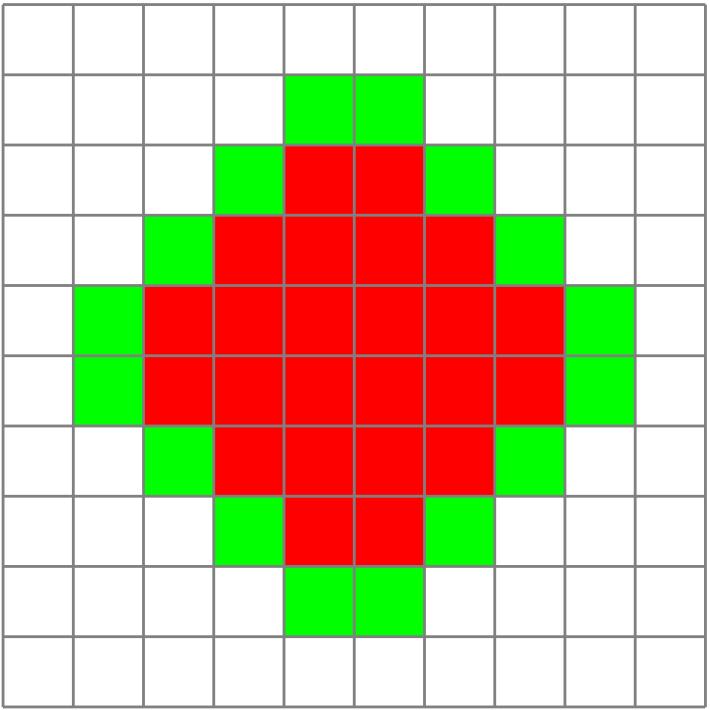
\includegraphics[width=0.4\linewidth]{Chapter4/figures/front_penny.png}
    \caption{Penny shaped crack discretized in a coarse grid. Red elements represent the fractured elements (which contain EFEM enrichments). The fracture front elements are shown in green. }
    \label{fig:crack_front}
\end{figure}

\begin{figure}
    \floatsetup[subfigure]{style=plain,capposition = beside, capbesideposition={left, center},capbesidesep=quad, capbesidewidth =5cm, captionskip=20pt, rowpostcode=captionskip}
    \captionsetup[subfloatrow]{format=hang, labelfont=up, textfont=up}
    \captionsetup{labelfont=sc}
    \ffigbox{%
      \begin{subfloatrow}[1]
        \fcapside{\caption{Beginning of time step. The phase-field fracture is shown as a countor to facilitate the visualization. As in \ref{fig:crack_front}, green elements represent the front and red the discrete fracture.}}
        {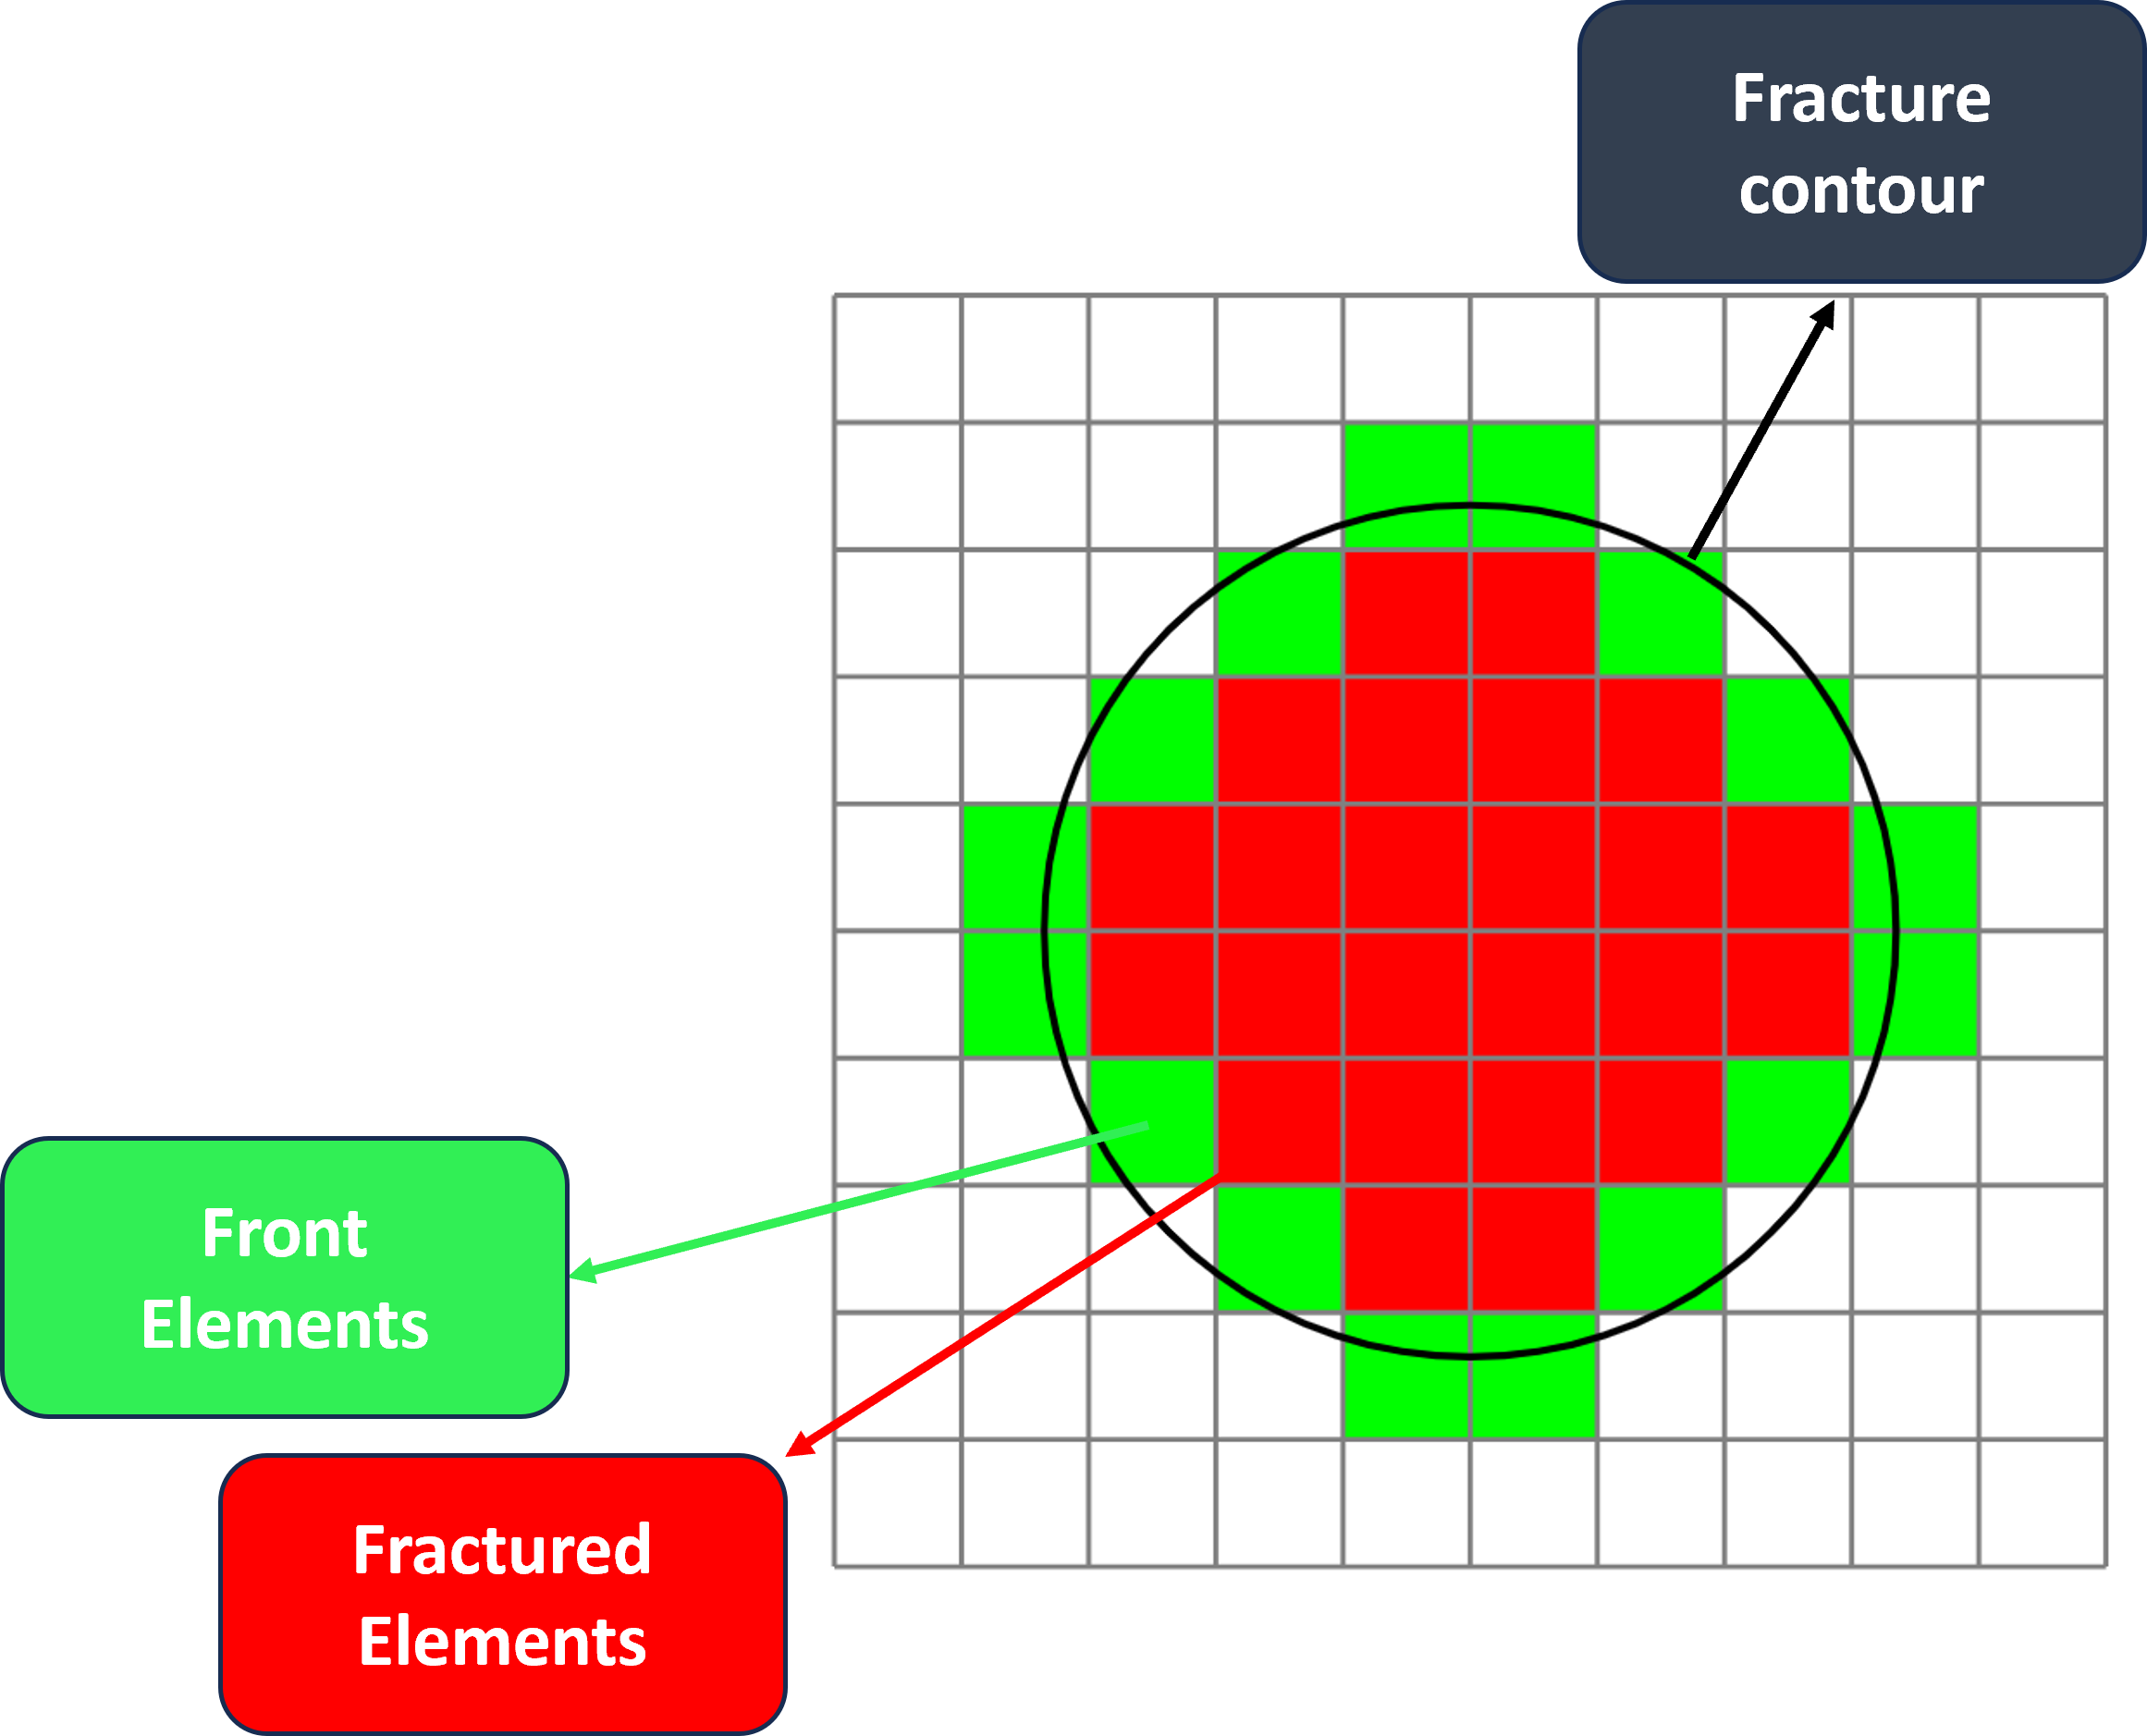
\includegraphics[width=\linewidth]{Chapter4/figures/penny_with_descriptions.png}}
      \end{subfloatrow}\\
      \begin{subfloatrow}[1]
        \fcapside{\hspace*{0.25cm}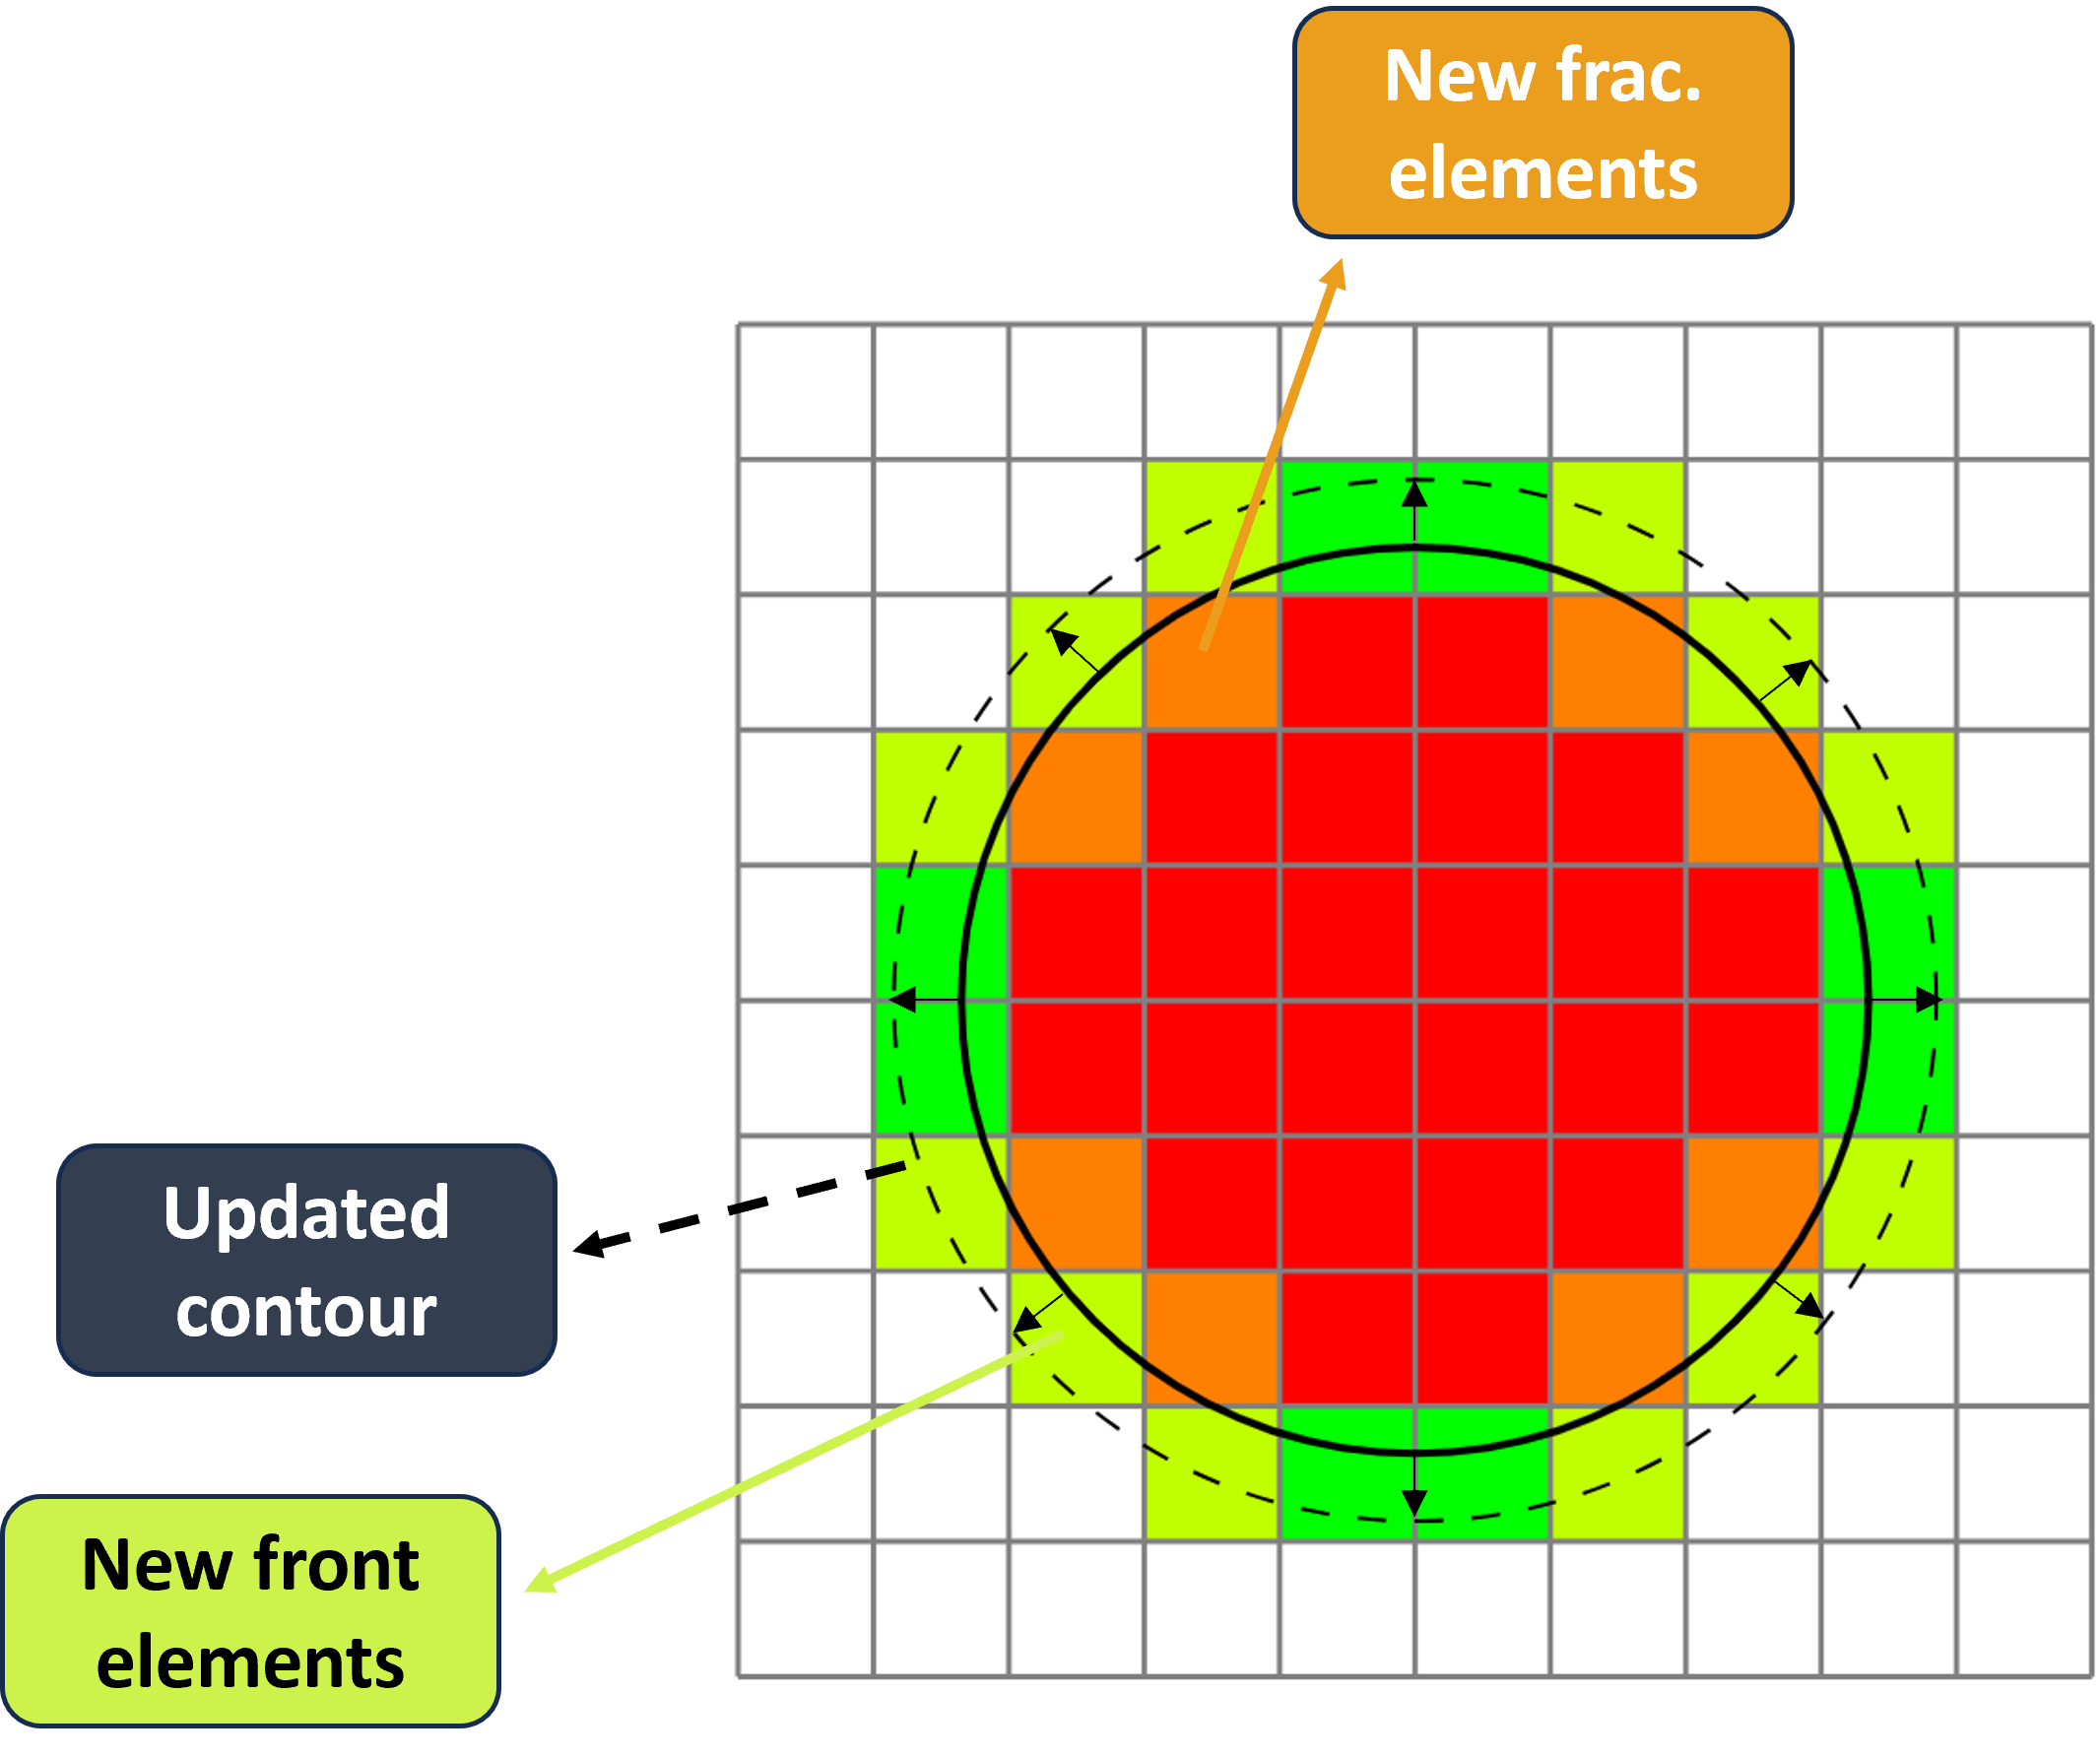
\includegraphics[width=0.9\linewidth]{Chapter4/figures/larger_penny_with_descriptions.png}}
        {\caption{After a few iterations in the local problem, the phase-field advances and some front elements (now in orange) are identified as fully damaged. They will be fractured and their neighbors in light green will be added to the front.}}
      \end{subfloatrow}\\
      \begin{subfloatrow}[1]
        \fcapside{\hspace*{2.60cm}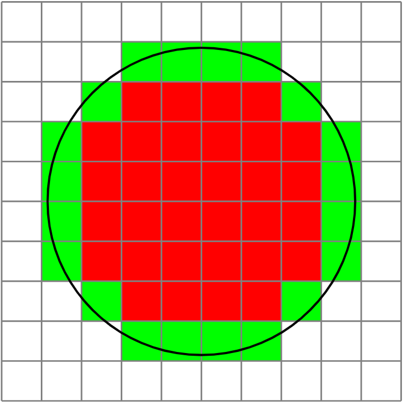
\includegraphics[width=0.6\linewidth]{Chapter4/figures/larger_penny.png}}
        { \caption{Final configuration after the updates. Since the global fracture changed, the time-step must be relaunched.}}
      \end{subfloatrow}\\
      }{\caption{Sequence of steps performed during crack propagation.}
      \label{fig:crack_prop_steps}}
  \end{figure}

\FloatBarrier

\subsection{Tracking damage in the fracture front elements}\label{frontTrackingAlgo}

The process of tracking the damage in the front elements also deserves a more detailed explanation. First, a simplified criterion suitable for planar cracks in structured grids is detailed. This is the one that is used in the preliminary results shown next. Then, a more general approach that can be used for unstructured meshes is described.

\subsubsection{Volume of damage criterion}

For this criterion, consider a structured grid, aligned with the coordinate axis and with the fracture planes. Suppose that a given element in the global domain has has dimensions $H_x, H_y$ and $H_z$ whereas the local one has $h_x, h_y$ and $h_z$.

Ths criterion begins by first computing the cross sectional area of that element along the fracture plane. For example, for a fracture whose normal is in the x direction, one gets $H_yH_z$. This is only possible when the structured grid is aligned with the fracture (either in $x, y$ or $z$).

Then, assuming that the fully damaged region of a phase-field fracture consists of a single element across the damage band width, the volume of the fully-cracked region can be estimated to be $h_xH_yH_z$ when the damage complete crosses the element. So, to check if that has happened, the volume of local elements with damage above a threshold (consider 0.9) is computed from the local problem solution. A global element is then considered fractured if this volume reaches $h_xH_yH_z$.

This method contains multiple limitations, such as the need for planar fractures aligned with a structured grid and also the hypothesis that the damage band has a single fully degraded element along its width. However, in many practical applications, the fractures are indeed assumed to be parallel to each other and structured grids are also preferred, as they can substantially reduce memory use. 

\subsubsection{Topological criterion}

An alternative method to circumvent these limitation is inspired by \cite{muixi2021combined}. It consists of evaluating the damage field in the edges of an element. It assumes that a fractured element has at least three fractured faces and that a fractured face is cut on two of its edges.

For each global element in the crack front, the damage field, computed in the local mesh, is inspected on every edge. If damage above a threshold (typically 0.9 or 0.95) is identified in a given edge, that edge is considered cut. If any face contains two cut edges, it is marked as cut. An element is then marked as fracture when at least three of its faces are cut.

This criteria circumvents some of the limitations of the simplified one, removing the need for structured grids. It is also applicable to non-planar fractures as well. However, it is not perfectly robust and certain relative configurations between the damage field and the global element in the front can lead to unexpected results. This will be shown in Section \ref{section: Chapter4/nonplanar} that discusses the case of non-planar fractures.
